\documentclass{beamer}
\usetheme{metropolis}
\usepackage{graphicx}
\usepackage{amsmath}
\usepackage{url}

\def\rcurs{{\mbox{$\resizebox{.16in}{.08in}{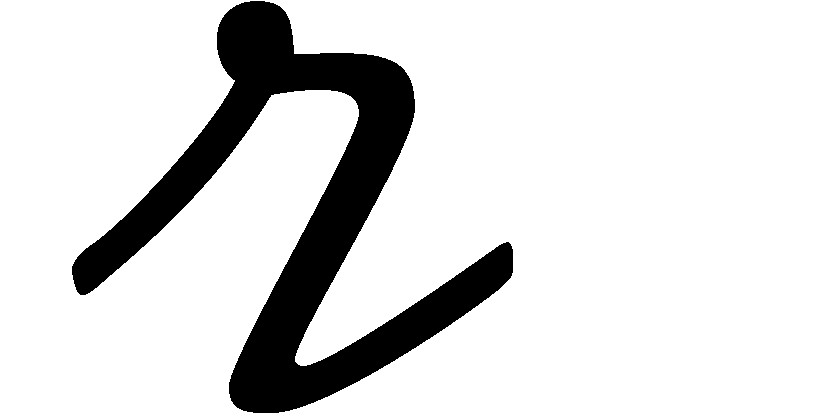
\includegraphics{ScriptR}}$}}}
\def\brcurs{{\mbox{$\resizebox{.16in}{.08in}{
\includegraphics{BoldR}}$}}}
\def\hrcurs{{\mbox{$\hat \brcurs$}}}

\title{Electromagnetc Theory: PHYS330}
\author{Jordan Hanson}
\institute{Whittier College Department of Physics and Astronomy}

\begin{document}
\maketitle

\section{Summary}

\begin{frame}{Week 5 Summary}
\begin{enumerate}
\item Current density and continuity equation
\item The divergence and curl of $\vec{B}$-fields
\item The magnetic vector potential, $\vec{B} = \nabla \times \vec{A}$
\begin{itemize}
\item Vector calculus theorems
\item Boundary conditions
\item Multipole expansion
\end{itemize}
\item Magnetic fields in matter
\begin{itemize}
\item Magnetization
\item Field of a magnetized object
\item The auxiliary field, $\vec{H}$
\item Linear magnetic media
\end{itemize}
\end{enumerate}
\end{frame}

\section{Current density and continuity equation}

\begin{frame}{Current density and continuity equation}
Let the \textit{current density} $\vec{J}$ be defined by
\begin{equation}
\vec{J} = \rho \vec{v}
\end{equation}
Units: current per unit area (other definitions available for different geometries).  So it's reasonable to obtain the whole scalar current by integrating:
\begin{equation}
I = \int_{\mathcal{S}} \vec{J} \cdot d\vec{a}
\end{equation}
If we want to account for the charge leaving a volume $\mathcal{V}$ through a closed surface $\mathcal{S}$ is
\begin{align}
\oint_{\mathcal{S}} \vec{J} \cdot d\vec{a} &= \int_{\mathcal{V}} (\nabla \cdot \vec{J}) d\tau \\
\int_{\mathcal{V}} (\nabla \cdot \vec{J}) d\tau &= -\frac{d}{dt} \int_{\mathcal{V}} \rho d\tau = -\int_{\mathcal{V}} \frac{\partial \rho}{\partial t} d\tau
\end{align}
\end{frame}

\begin{frame}{Current density and continuity equation}
This is true for \textit{any} volume, so the integrands must be equal:
\begin{equation}
\nabla \cdot \vec{J} = -\frac{\partial \rho}{\partial t}
\end{equation}
This is called the continuity equation, and it also arises in quantum mechanics.  If $\partial\rho/\partial t = 0$, then we have a \textbf{steady current.} \\ \vspace{0.5cm}
Suppose we have a current density $\vec{J}(\vec{r}) = I_0(t) \hat{r}/r^2$, with $I_0(t) = \delta(t-t_0)$.  Find $\rho(t)$, the charge density as a function of time in the region containing $\vec{J}$. (Breakout rooms).
\end{frame}

\section{The Divergence of $B$-fields}

\begin{frame}{The Divergence of $B$-fields}
The Biot-Savart law states that
\begin{equation}
\vec{B}(\vec{r}) = \frac{\mu_0}{4\pi} \int \frac{\vec{J}(\vec{r'}) \times \hrcurs }{\rcurs} d\tau'
\end{equation}
\begin{figure}
\centering
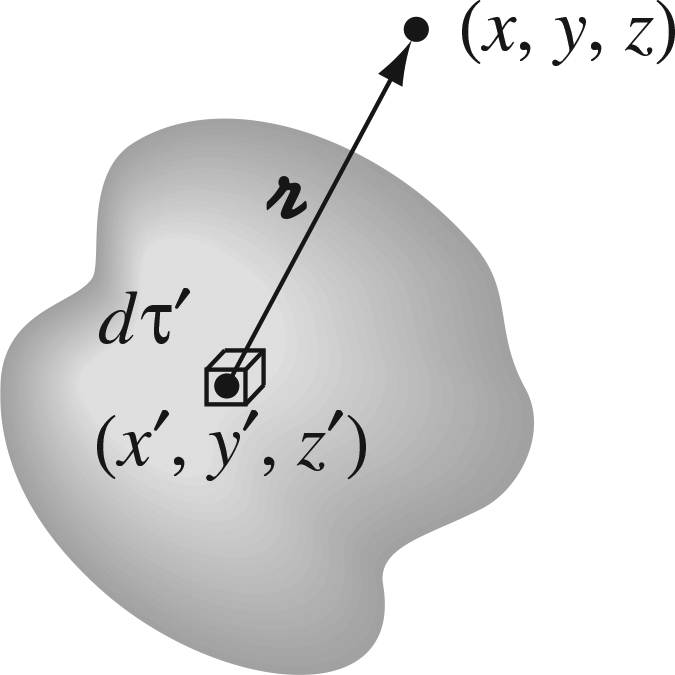
\includegraphics[width=3cm]{figures/5_30.png}
\caption{\label{fig:biot} Definitions of coordinates in variables for derivation of divergence of B-fields.  The gray region represents charges and current densities.}
\end{figure}
\end{frame}

\begin{frame}{The Divergence of $B$-fields}
Take the divergence of the Biot-Savart law, but then use a product rule for the integrand.
\begin{align}
\nabla \cdot \vec{B} =& \frac{\mu_0}{4\pi} \int \nabla \cdot \left( \vec{J} \times \frac{\hrcurs}{\rcurs^2}\right) d\tau' \\
\nabla \cdot \left( \vec{J} \times \frac{\hrcurs}{\rcurs^2}\right) &= \frac{\hrcurs}{\rcurs^2} \cdot (\nabla \times \vec{J}) - \vec{J} \cdot \left( \nabla \times \frac{\hrcurs}{\rcurs^2} \right)
\end{align}
\begin{itemize}
\item $\nabla \times \vec{J} = 0$, because this is like taking $df(x)/dx'$.
\item We showed in Chapter 1 that $\nabla \times \frac{\hrcurs}{\rcurs^2} = 0$.  Is this visually obvious?
\end{itemize}
Thus,
\begin{equation}
\boxed{
\nabla \cdot \vec{B} = 0
}
\end{equation}
\end{frame}

\begin{frame}{The Divergence of $B$-fields}
From warmup exercises, we know that we can therefore write
\begin{equation}
\vec{B} = \nabla \times \vec{A}
\end{equation}
(Breakout rooms): create three divergence-less vector fields.  One in Cartesian coordinates, one in cylindrical coodinates, and one in spherical.  Exclude trivial cases like $\vec{B} = 0$.
\end{frame}

\section{The Curl of $\vec{B}$-fields}

\begin{frame}{The Curl of $\vec{B}$-fields}
Because $\vec{B}$-fields have no divergence, we can write
\begin{equation}
\vec{B} = \nabla \times \vec{A}
\end{equation}
Because the curl of the gradient of a scalar function is zero, we can choose\footnote{We can always find a scalar function whose gradient we are free to add to $\vec{A}$ that makes the divergence go away.}
\begin{equation}
\nabla \cdot \vec{A} = 0
\end{equation}
Since $\nabla \times (\nabla \times \vec{A}) = \nabla(\nabla \cdot \vec{A}) - \nabla^2 \vec{A} = \mu_0 \vec{J}$,
\begin{equation}
\boxed{
\nabla^2 \vec{A} = -\mu_0 \vec{J}
}
\end{equation}
\end{frame}

\begin{frame}{The Curl of $\vec{B}$-fields}
Find the vector potential of an infinite solenoid with $n$ turns per unit length, radius $R$, and current $I$.
\begin{itemize}
\item First, what is $\vec{B}$, from Amp\`{e}re's Law?
\item Why can we \textit{not} just do this business, as with Poisson's equations for $V(\vec{r'})$?
\begin{equation}
\vec{A} = \frac{\mu_0}{4\pi	}\int \frac{\vec{J}(\vec{r'})}{\rcurs} d\tau' = \frac{\mu_0 I}{4\pi}\int \frac{1}{\rcurs} d\vec{l'}
\end{equation}
\item Notice that
\begin{equation}
\oint \vec{A} \cdot d\vec{l} = \int (\nabla \times \vec{A}) \cdot d\vec{a} = \int \vec{B} \cdot d\vec{a} = \Phi_B
\end{equation}
by Stoke's Theorem.
\item Obtain $\oint \vec{A} \cdot d\vec{l}$ Amp\`{e}rian loop of radius $s$, and $\vec{B}$ from Amp\`{e}re's Law ...
\end{itemize}
\end{frame}

\section{Boundary Conditions}

\begin{frame}{Boundary Conditions}
What boundary conditions exist for $\vec{B}$ and $\vec{A}$ at surface currents? \\ \vspace{0.25cm}
\textbf{$\vec{B}$-fields}
\begin{enumerate}
\item Review of a surface current, $\vec{B}$-field of a uniform surface current
\item Apply divergence theorem for $\vec{B}_{\perp}$
\item Apply Amp\`{e}re's Law for $\vec{B}_{||}$
\end{enumerate}
\textbf{$\vec{A}$-fields}
\begin{enumerate}
\item Divergence
\item $\oint \vec{A} \cdot d\vec{l}$
\end{enumerate}
\end{frame}

\begin{frame}{Boundary Conditions}
\begin{figure}
\centering
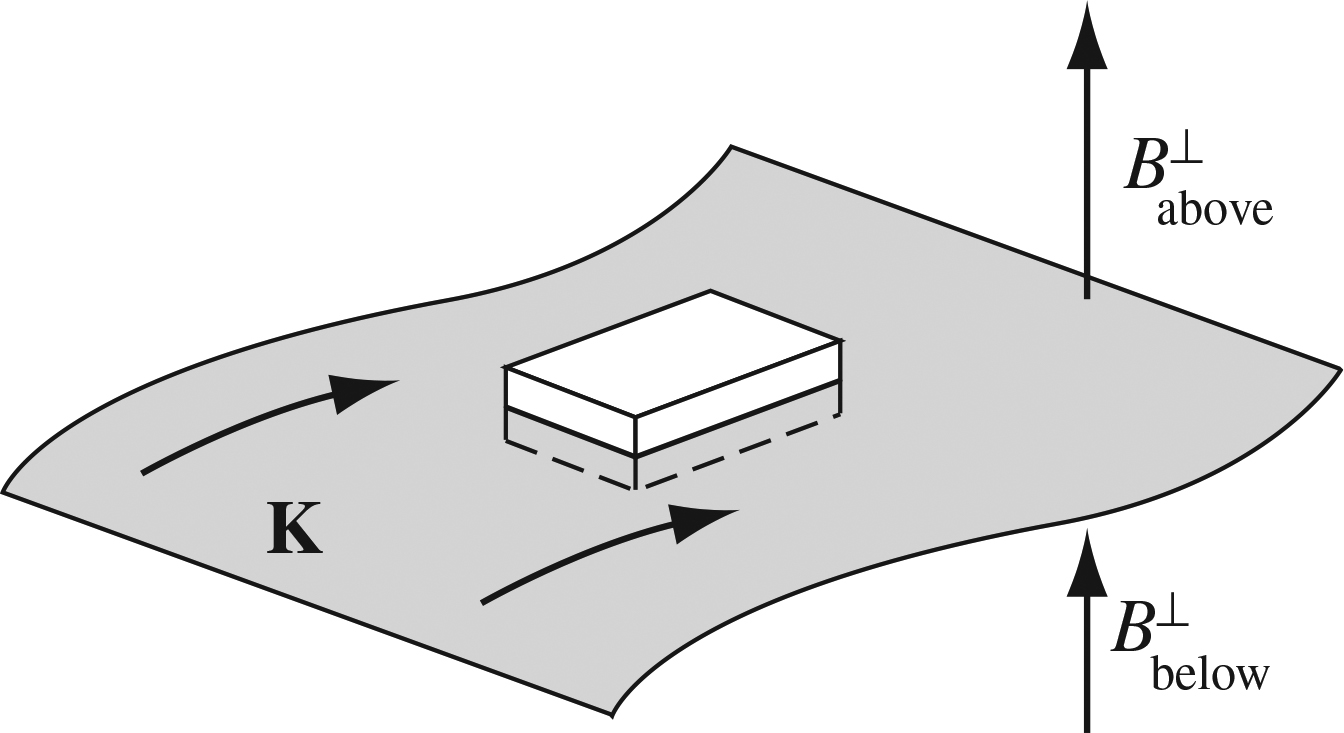
\includegraphics[width=5cm]{figures/5_49.jpg}
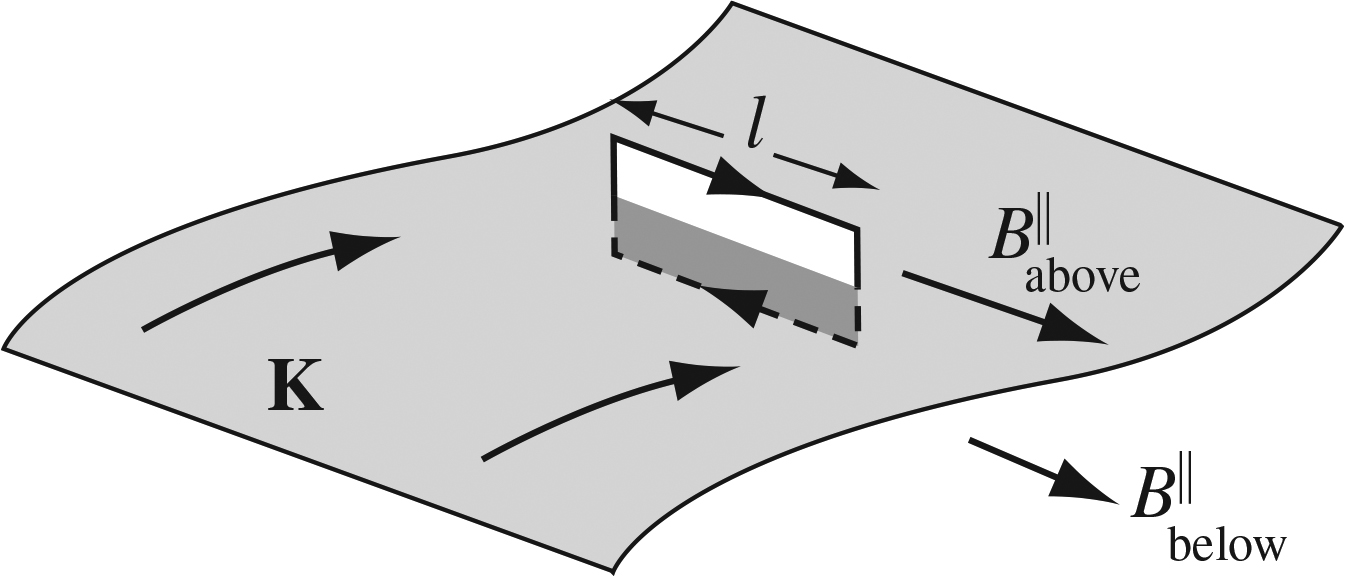
\includegraphics[width=5cm]{figures/5_50.jpg}
\caption{\label{fig:bound} (Left) Perpendicular B-field condition (Right) Parallel B-field condition.}
\end{figure}
\end{frame}

\section{Multipole Expansion for Vector Potential}

\begin{frame}{Multipole Expansion for Vector Potential}
It's still true that the generator function for the Legendre polynomials is $1/\rcurs$:
\begin{equation}
\frac{1}{\rcurs} = \frac{1}{r}\sum_{n=0}^{\infty} \left(\frac{r'}{r}\right)^n P_n(\cos\alpha)
\end{equation}
(Remember that $\alpha$ is the angle between $r$ and $r'$).  Therefore for any current loop:
\begin{align}
\vec{A} &= \frac{\mu_0 I}{4\pi} \oint \frac{1}{\rcurs} d\vec{l} \\
\vec{A} &= \frac{\mu_0 I}{4\pi} \sum_{n=0}^{\infty} \frac{1}{r^{n+1}} \oint (r')^n P_n(\cos\alpha) d\vec{l} \label{eq:multA}
\end{align}
\end{frame}

\begin{frame}{Multipole Expansion for Vector Potential}
\alert{\textbf{Use Eq. \ref{eq:multA}}} to find the $n = 0$ and the $n = 1$ terms.
\begin{enumerate}
\item Can you explain the result for the $n = 0$ term on physical grounds?
\item Show that the second term is
\begin{equation}
\vec{A}(\vec{r}) = \frac{\mu_0 I}{4\pi r^2} \oint r' \cos\alpha d\vec{l'}
\end{equation}
\item Convince yourself that $\hat{r} \cdot \vec{r'} = r' \cos\alpha$.
\item Now we're going on a trip down memory lane...
\end{enumerate}
\end{frame}

\begin{frame}{Multipole Expansion for Vector Potential}
Recall from the Ch. 1 homework that
\begin{equation}
\oint (\vec{c} \cdot \vec{r'}) d\vec{l'} = \vec{a} \times \vec{c}
\end{equation}
where $\vec{a}$ is the ``area vector.''
\begin{equation}
\vec{a} = \int_{\mathcal{S}} d\vec{a'}
\end{equation}
The vector field $\vec{c}$ is a constant one.  Let $\vec{c} = \hat{r}$ to find
\begin{equation}
\oint (\hat{r} \cdot \vec{r'}) d\vec{l'} = \vec{a} \times \hat{r}
\end{equation}
\end{frame}

\begin{frame}{Multipole Expansion for Vector Potential}
Putting it all together for the $n = 1$ term:
\begin{equation}
\vec{A}_{dipole}(\vec{r}) = \frac{\mu_0}{4\pi} \frac{\left(I \int_{\mathcal{S}} d\vec{a'}\right) \times \hat{r}}{r^2}
\end{equation}
Define the vector $\vec{m}$ as
\begin{equation}
\vec{m} = I \int_{\mathcal{S}} d\vec{a'}
\end{equation}
So that
\begin{equation}
\boxed{
\vec{A}_{dipole}(\vec{r}) = \frac{\mu_0}{4\pi} \frac{\vec{m} \times \hat{r}}{r^2}
}
\end{equation}
\end{frame}

\begin{frame}{Multipole Expansion for Vector Potential}
\begin{figure}
\centering
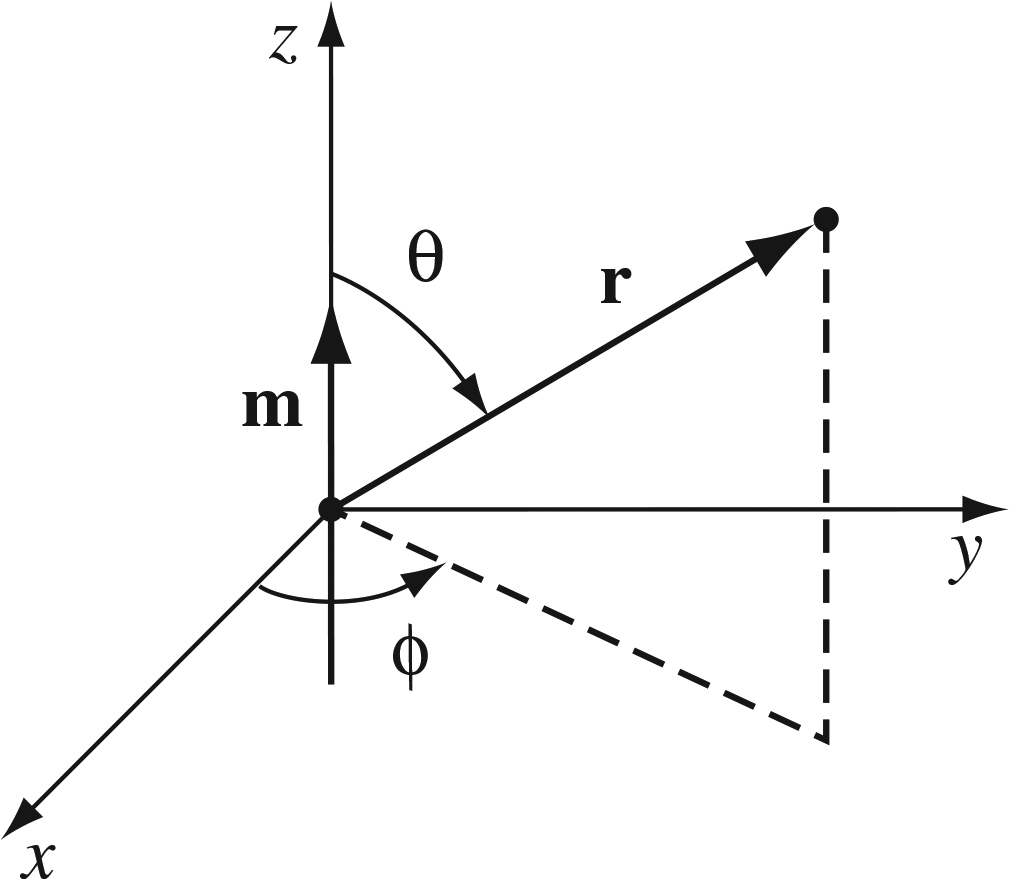
\includegraphics[width=5cm]{figures/5_54.jpg}
\caption{\label{fig:mdip} Choose this geometry for the magnetic dipole.}
\end{figure}
\begin{enumerate}
\item Evaluate the dipole term for the vector potential with this geometry
\item Compute the curl
\end{enumerate}
\end{frame}

\section{Conclusion}

\begin{frame}{Week 5 Summary}
\begin{enumerate}
\item Current density and continuity equation
\item The divergence and curl of $\vec{B}$-fields
\item The magnetic vector potential, $\vec{B} = \nabla \times \vec{A}$
\begin{itemize}
\item Vector calculus theorems
\item Boundary conditions
\item Multipole expansion
\end{itemize}
\item Magnetic fields in matter
\begin{itemize}
\item Magnetization
\item Field of a magnetized object
\item The auxiliary field, $\vec{H}$
\item Linear magnetic media
\end{itemize}
\end{enumerate}
\end{frame}

\end{document}
